\documentclass[12pt,blue]{beamer}
\usepackage{beamerthemesplit}
\usepackage{beamerthemeshadow}
\usepackage{animate}
\usepackage[3D]{movie15}
\usepackage{hyperref}
%\usepackage[numbered]{mcode}
\usepackage{graphics}
\usepackage{pgf,pgfarrows,pgfnodes,pgfautomata,pgfheaps}
\usepackage{amsmath,amssymb}
\usepackage{pgfpages}
%\setbeameroption{show only notes}
%\setbeameroption{show notes on second screen=right}
\usepackage{tikz}
\usetikzlibrary{trees}
\usetikzlibrary{decorations.pathmorphing}
\usetikzlibrary{decorations.markings}


\usetheme{Warsaw}

\usecolortheme{sidebartab}
%beetle,crane,dove,fly,seagull,wolverine,beaver
\renewcommand{\raggedright}{\leftskip=0pt \rightskip=0pt plus 0cm}
\raggedright
\graphicspath{{figures/}}
\definecolor{MyDarkGreen}{rgb}{0.0,0.4,0.0}


%%%%%%%%%%%%%%%%%%%%%%%%%%%%%%%%%%%%%%%%%%%%%%%%%%%%%%
\usepackage{xeCJK}
\usepackage{fontspec}
\setCJKmainfont[BoldFont=simhei.ttf]{simkai.ttf}
%\setCJKsansfont{simhei.ttf}
%\setCJKmonofont{simfang.ttf}

%%%%%%%%%%%%%%%%%%%%%%%%%%%%%%%%%%%%%%%%%%%%%%%%%%%%%%%%%%%%%%%%%%%%%%%%%%
\makeatletter
\usefoottemplate{ %重新定义页脚,加入作者,单位,单位图标,和文档标题
  \vbox{\tiny%
    \hbox{%
      \setbox\beamer@linebox=\hbox to\paperwidth{%
        \hbox to.5\paperwidth{
            \hfill\tiny\color{white}
                  \textbf{\insertshortauthor\quad\insertshortinstitute}
            \hskip .1cm\lower 0.2em\hbox{
\includegraphics[height=0.25cm]{./figures/CAS.pdf}}
            \hskip.3cm}%
        \hbox to.5\paperwidth{
            \hskip.3cm\tiny\color{white}
                  \textbf{\insertshorttitle}\hfill}\hfill}%
      \ht\beamer@linebox=2.625ex%
      \dp\beamer@linebox=0pt%
      \setbox\beamer@linebox=\vbox{\box\beamer@linebox\vskip1.125ex}%
      \color{structure}\hskip-\Gm@lmargin\vrule width.5\paperwidth
      height\ht\beamer@linebox\color{structure!70}\vrule width.5\paperwidth
      height\ht\beamer@linebox\hskip-\paperwidth%
      \hbox{\box\beamer@linebox\hfill}\hfill\hskip-\Gm@rmargin}
  }
}
\makeatother
%%%%%%%%%%%%%%%%%%%%%%%%%%%%%%%%%%%%%%%%%%%%%%%%%%%%%%%%%%%%%%%%%%%%%%%%%%

\begin{document}


\title{文献阅读}
\subtitle{组会}
\author[周吕文]{周吕文}

\institute[中国科学院力学研究所,LHO]{中国科学院力学研究所,LHO}
\date{October 24, 2010}
\subject{Computer Tools, TeX, Slide}
%\titlegraphic{\pgfuseimage{title}}

\frame[plain]{\titlepage}
\AtBeginSection[]{ % 在每个Section前都会加入的Frame
  \frame<handout:0>{
    \frametitle{Outline}
    \tableofcontents[current,currentsubsection]
  }
}

\part{Self-consistent dissipative particle dynamics algorithm}
\frame{\partpage}

\section{欧拉法(Euler)}
\frame{\frametitle{欧拉法}

欧拉法速度和位置的更新如下:

\[
r_i(t+\Delta t) = r_i(t) + v_i(t)\Delta t
\]

\[
v_i(t+\Delta t) = v_i(t) +f_i(t)\Delta t
\]

\[
f_i(t+\Delta t) = f_i\Big(r_i(t+\Delta t), v_i(t+\Delta t)\Big)
\]
}

\frame{\frametitle{欧拉法的缺点}

欧拉法的缺点:
\begin{itemize}
\item 时间步长对体系的平恒特征有影响。比如仿真中理想耗散气体系统的温度。
\[
mk_BT_{eq} = \frac{A_3}{A_1(2-A_1n\Delta t) - A_2\Delta t}
\footnote{Dissipative particle dynamics: The equilibrium for finite time steps. C. A. Marsh and J. M. Yeomans. Europhys. Lett. 37(8), pp. 511-516 (1997)}
\]
其中, $A_1=\frac{\gamma}{md}[w_D]$, $A_2 = \frac{2\gamma^2}{m^2d}[w_D^2]$ $A_3=\frac{\sigma^2}{d}[w_R^2]$
\item 时间步长对径向分布函数有影响。
\item 时间不可逆。
\end{itemize}
}

\section{跳蛙法(leap-frog)}
\frame{\frametitle{跳蛙法(leap-frog)}

跳蛙法(leap-frog)速度和位置的更新如下:

\[
v_i\Big(t+\frac{\Delta t}{2}\Big) = v_i\Big(t-\frac{\Delta t}{2}\Big) + \Delta t\frac{f_i(t)}{m}
\]

\[
r_i(t+\Delta t) = r_i(t) + v_i(t)\Delta t + f_i(t)\frac{(\Delta t)^2}{2m}
\]
}

\frame{\frametitle{跳蛙法的特点}

跳蛙法的特点:
\begin{itemize}
\item 自洽(self-consistently)
\item 时间可逆(time reversible)。
\item 仿真的时间步长不再受算法限制。
\item 计算量更大,需要更多开销。
\end{itemize}
}


\section{算例对比}
\frame{\frametitle{算例对比}

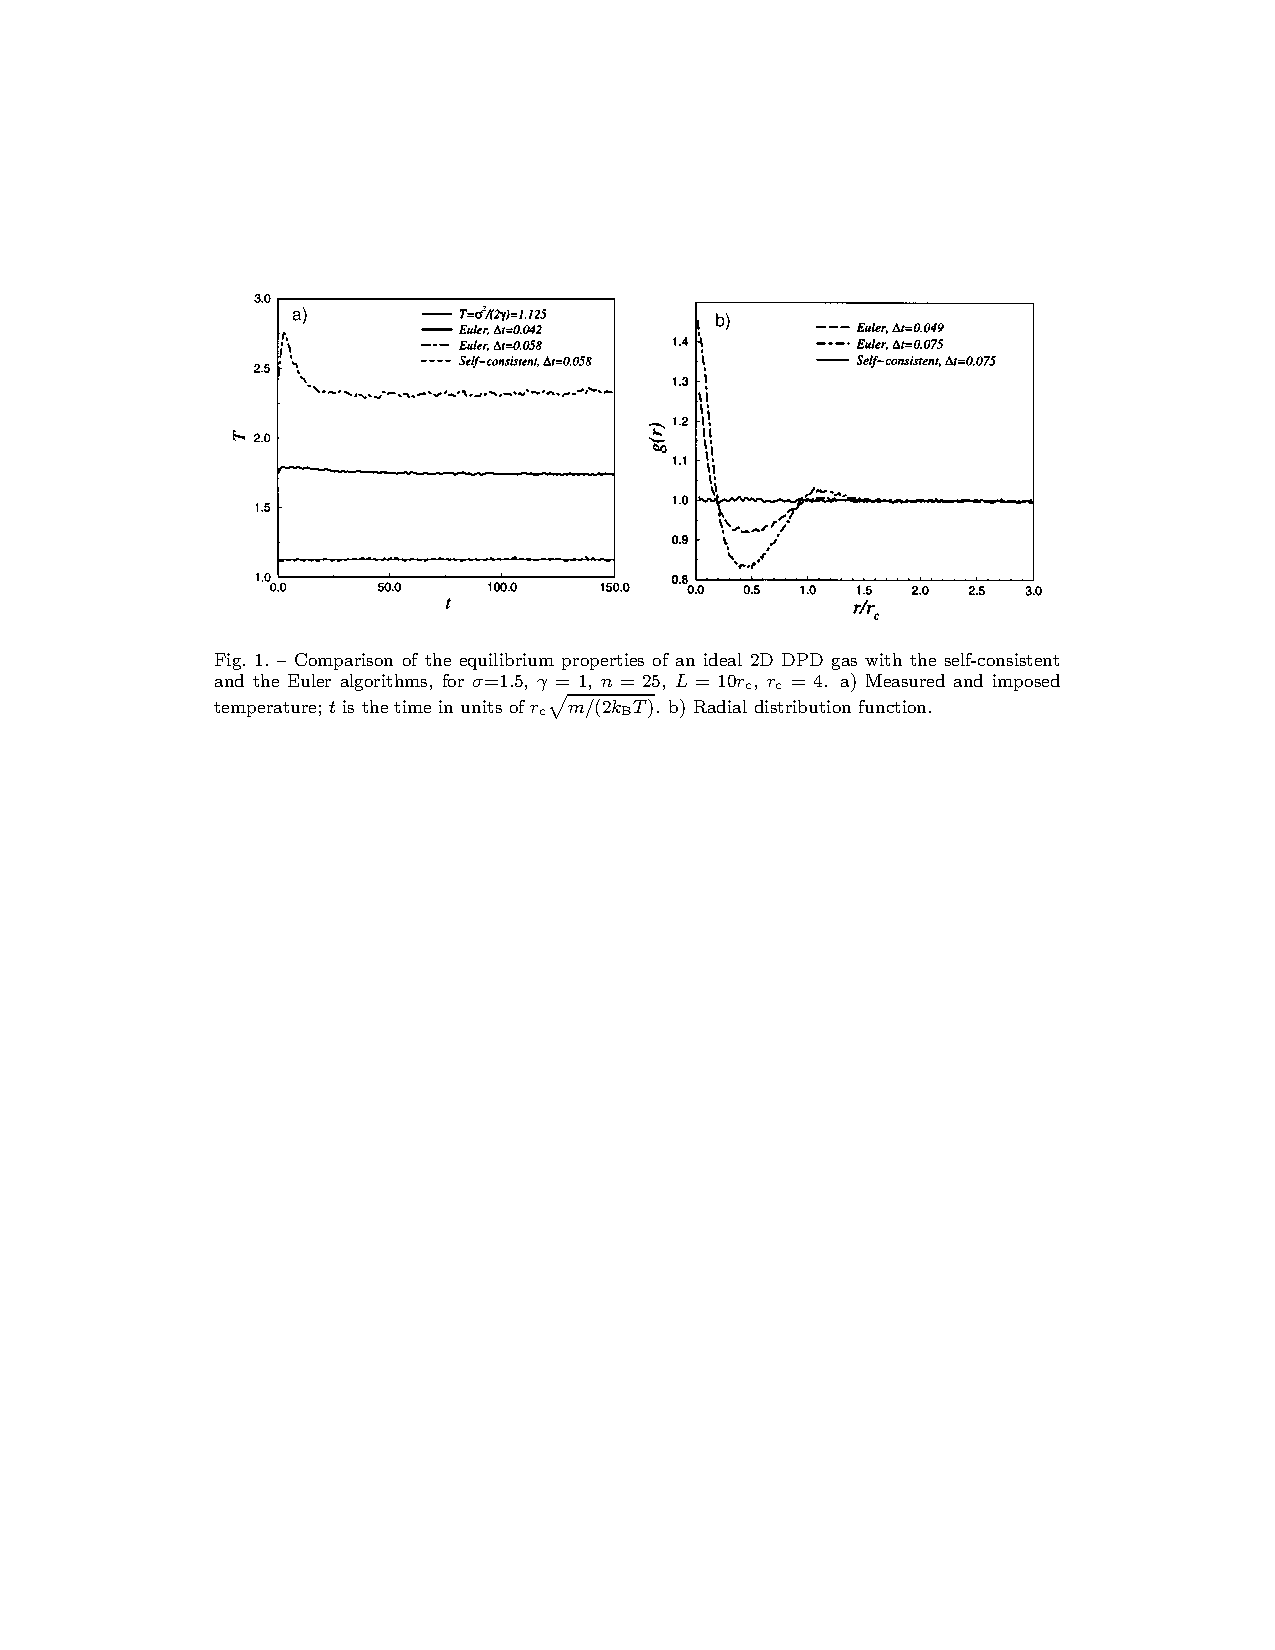
\includegraphics[width=\textwidth]{./figures/Comparison.pdf}
}


\part{Dissipative-particle-dynamics model for two-phase flows}
\frame{\partpage}

\section{两相的DPD模型}
\frame{\frametitle{DPD与分子动力学的差别}

\begin{columns}
\begin{column}[c]{0.5\textwidth}
\begin{center}
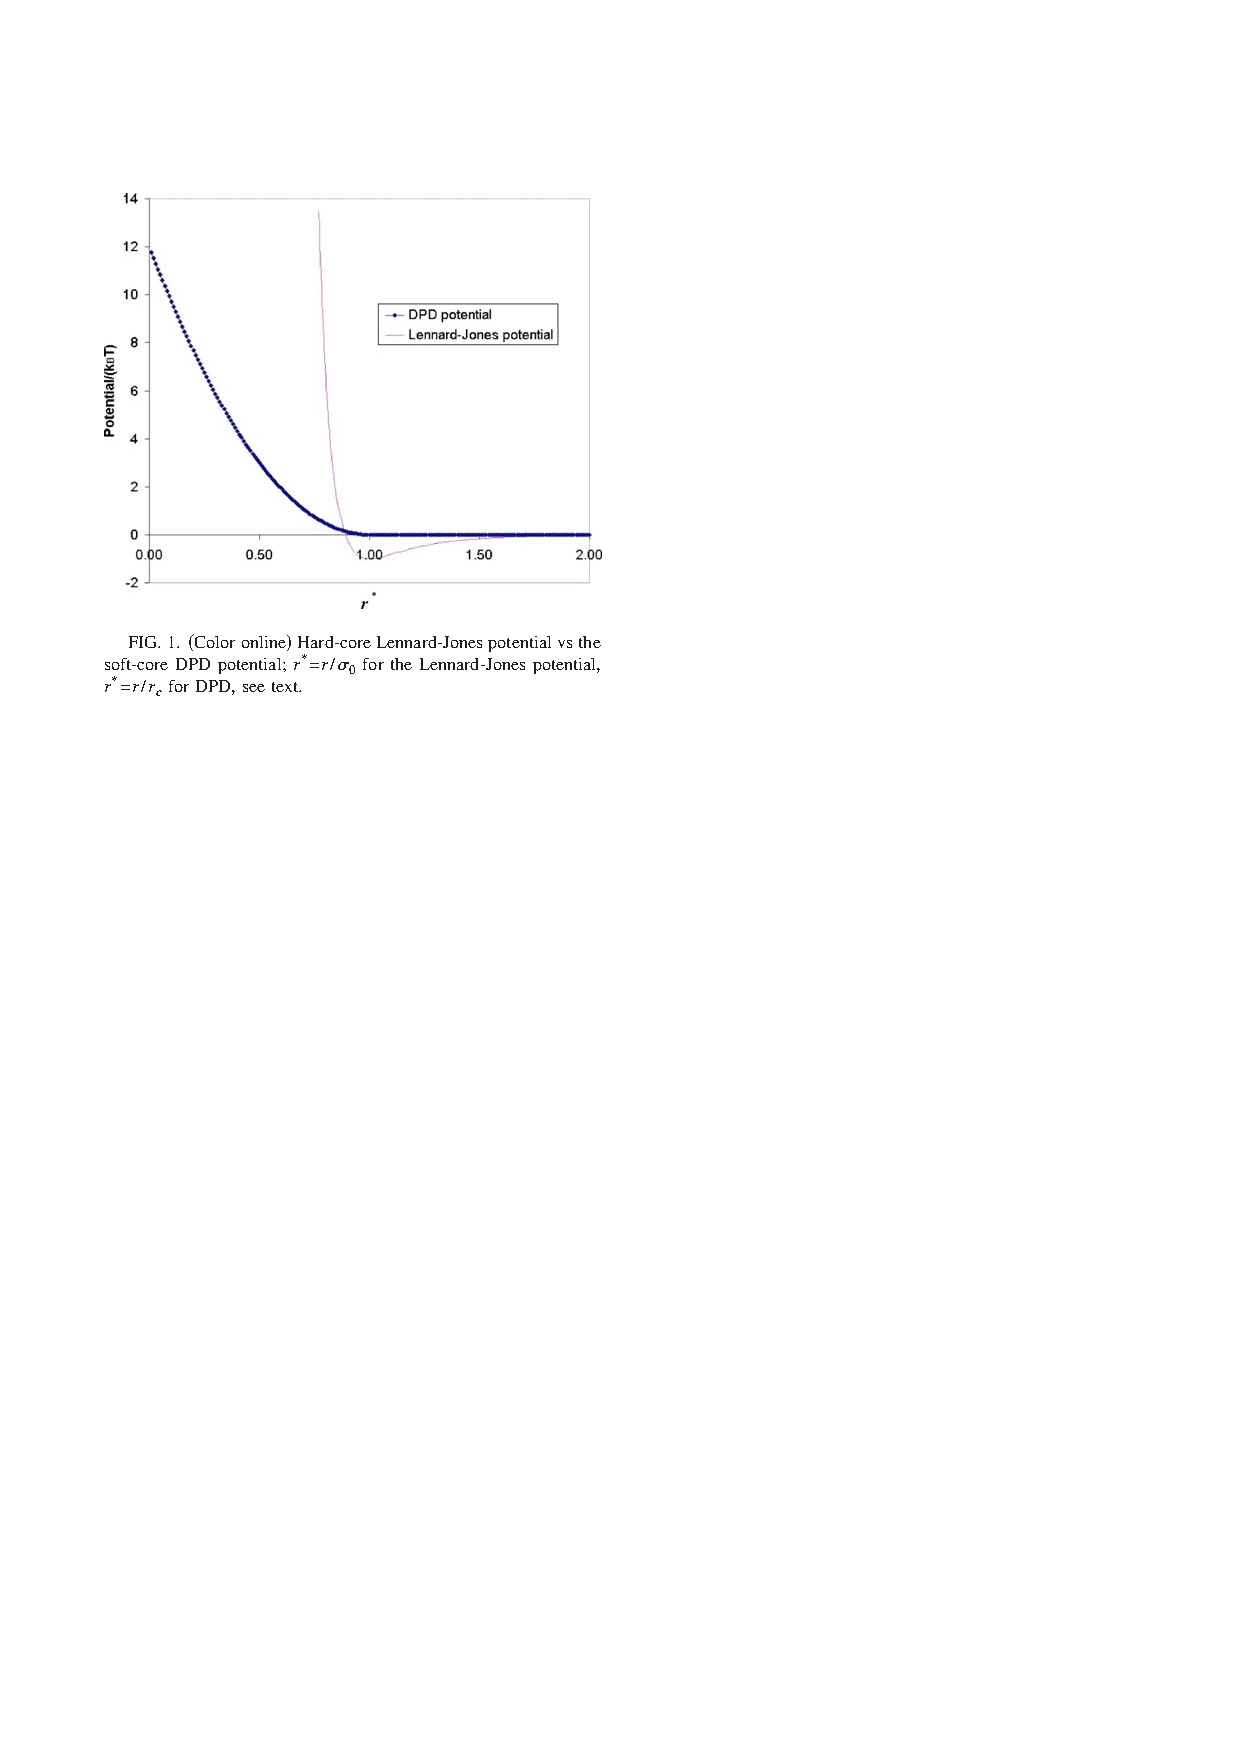
\includegraphics[width=\textwidth]{./figures/PotentialVsR.pdf}
\end{center}
\end{column}
\begin{column}[c]{0.5\textwidth}
\begin{enumerate}
\item lennard-Jones 势能的斜率太陡,力的变化太快,因此对$\Delta t$的要求较高。
\item DPD 势能的斜率相对lennard-Jones 势能比较平缓。对应的守恒力
\[F_{ij}^C=a_{ij}(1-r_{ij}/r_c)e_{ij}\]
\end{enumerate}
\end{column}
\end{columns}
}

\frame{\frametitle{van der waals 状态方程}
\begin{columns}
\begin{column}[c]{0.5\textwidth}
\begin{center}
\includegraphics[width=\textwidth]<2->{./figures/van_der_Walls.pdf}
\end{center}
\end{column}
\begin{column}[c]{0.5\textwidth}
\begin{enumerate}
%\item<1-> 保守力可由自由导出:$\mathbf{F}_{ij}^C = - \frac{\partial \psi(r_{ij})}{\partial r_{ij}}\mathbf{e_{ij}}$
\item<1-> 耗散力和随机力反应流体力学的性质, 保守力表现热力学的性质。
\item<3-> 保守力\\$F_{ij}^C=a_{ij}(1-r_{ij}/r_c)e_{ij}$\\
  并不能体现表现表面张力的长程力。
 \item<4-> 能引起相分离和表面张力的保守力形式\\
 $F^C=-\nabla \psi_{nonideal}+F^S$
\end{enumerate}
\end{column}
\end{columns}
}

\frame{\frametitle{平均自由能及其泰勒展开}

每个粒子的平均自由能
\begin{equation}
\psi_m = \int u_{att}(r)\rho dr\ \  \underrightarrow{\textrm{泰勒展开}}
\ \ \psi_m = -a\rho - k\nabla^2\rho
\end{equation}

其中

\[
a = -\frac{1}{2}\int_{r>\sigma_0}u_{att}(r)dr, \ \ \ \kappa = -\frac{1}{6}\int_{r>\sigma_0}r^2u_{att}(r)dr
\]

}

\frame{\frametitle{基于van der waals 状态方程的自由能}

由van der waals 状态方程
\[
(p+\frac{n^2a}{V^2})(V-nb)=nRT \Longrightarrow p = \frac{\rho k_B T}{1-b\rho}-a\rho^2
\]

结合$p=\frac{\partial \psi}{\partial v}$ 可得

\begin{center}
$\psi = \underline{\textcolor{red}{-k_bT\ln(1-b\rho)-a\rho}}+\underline{\textcolor{blue}{k_BT\ln\rho}}$\\
\ \ \ \ \ \ \ \ \ \ $\textcolor{red}{\psi_{non-ideal}}$ \ \ \ \ \ \ \ \ \ \ \ \ \ \ \ $\textcolor{blue}{F^S}$
\end{center}
}

\frame{\frametitle{密度的计算}

密度的计算采用了SPH中密度计算的方法
\[
\rho_i=\sum_{j=1}^N w(r_{ij})
\]

其中$w$满足: $ \int_0^{r_{c}}2\pi rw(r)rdr = 1$, 二维的权函数$w$如下

\begin{displaymath}
w(r,r_C) = \left\{\begin{array}{ll}
\frac{5}{\pi r_C^2}(1+\frac{3r}{r_c})(1-\frac{r}{r_C})^3 & \textrm{if $r<r_c$}\\
0 & \textrm{if $r>r_c$}
\end{array} \right.
\end{displaymath}
}

\frame{\frametitle{保守力的最终表达式}

表面张力项

\[
F^S=\kappa \nabla\nabla^2\rho
\]

因此保守力为

\[
F^C=\nabla[k_bT\ln(1-b\rho)+a\rho]+\kappa\nabla\nabla^2\rho
\]

结合前面相关结果,最终得到

\[
f_{ij}^C=\Big[-\Big\{\big(\frac{bk_BT}{1-b\rho_i}\big)+\big(\frac{bk_BT}{1-b\rho_j}-a\big)\Big\}w_{ij}^{(1)}+\kappa w_{ij}^{(3)}\Big]
\]
}

\section{算例}
\subsection{Liquid layer simulations}

\frame{\frametitle{结构与参数}
\begin{columns}
\begin{column}[c]{0.5\textwidth}
\begin{center}
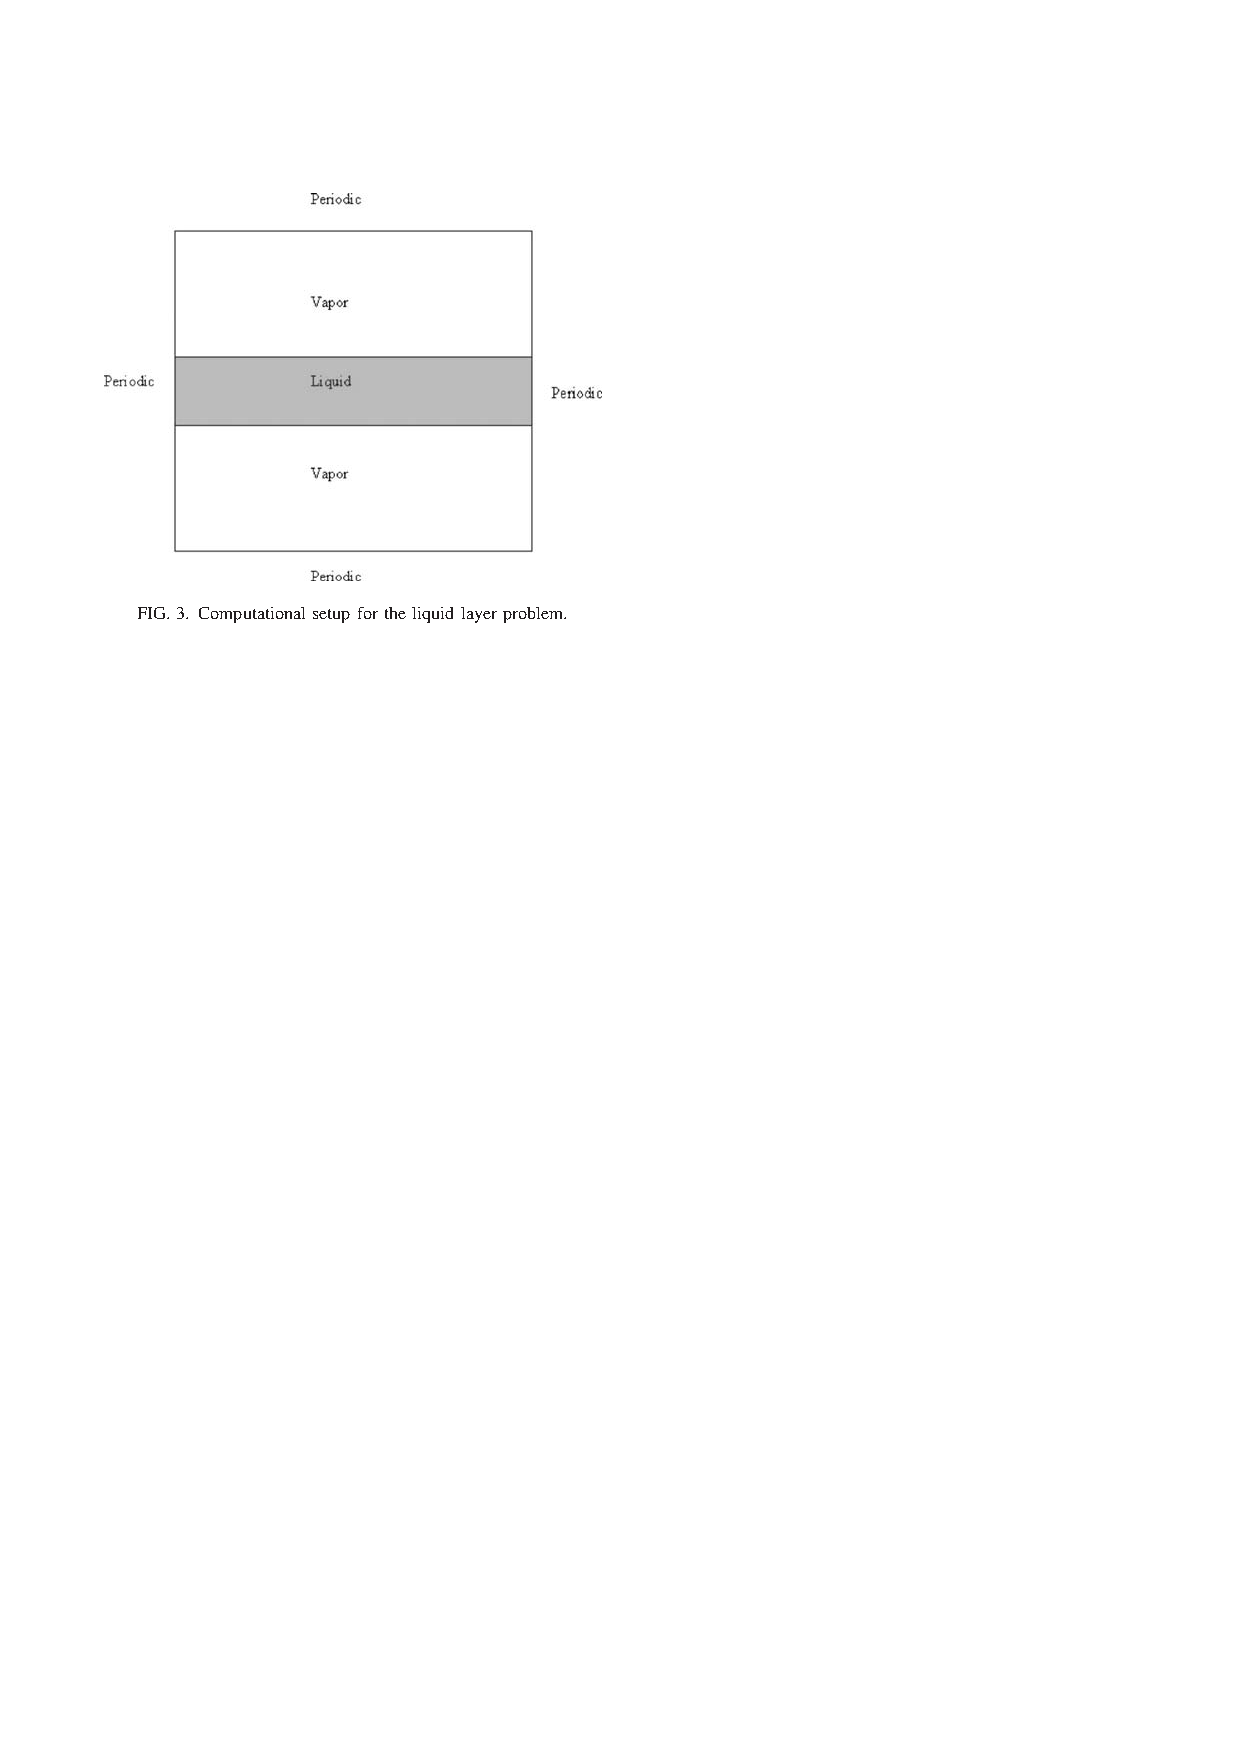
\includegraphics[width=1\textwidth]{./figures/configuration.pdf}
\end{center}
\end{column}
\begin{column}[c]{0.5\textwidth}
\begin{center}
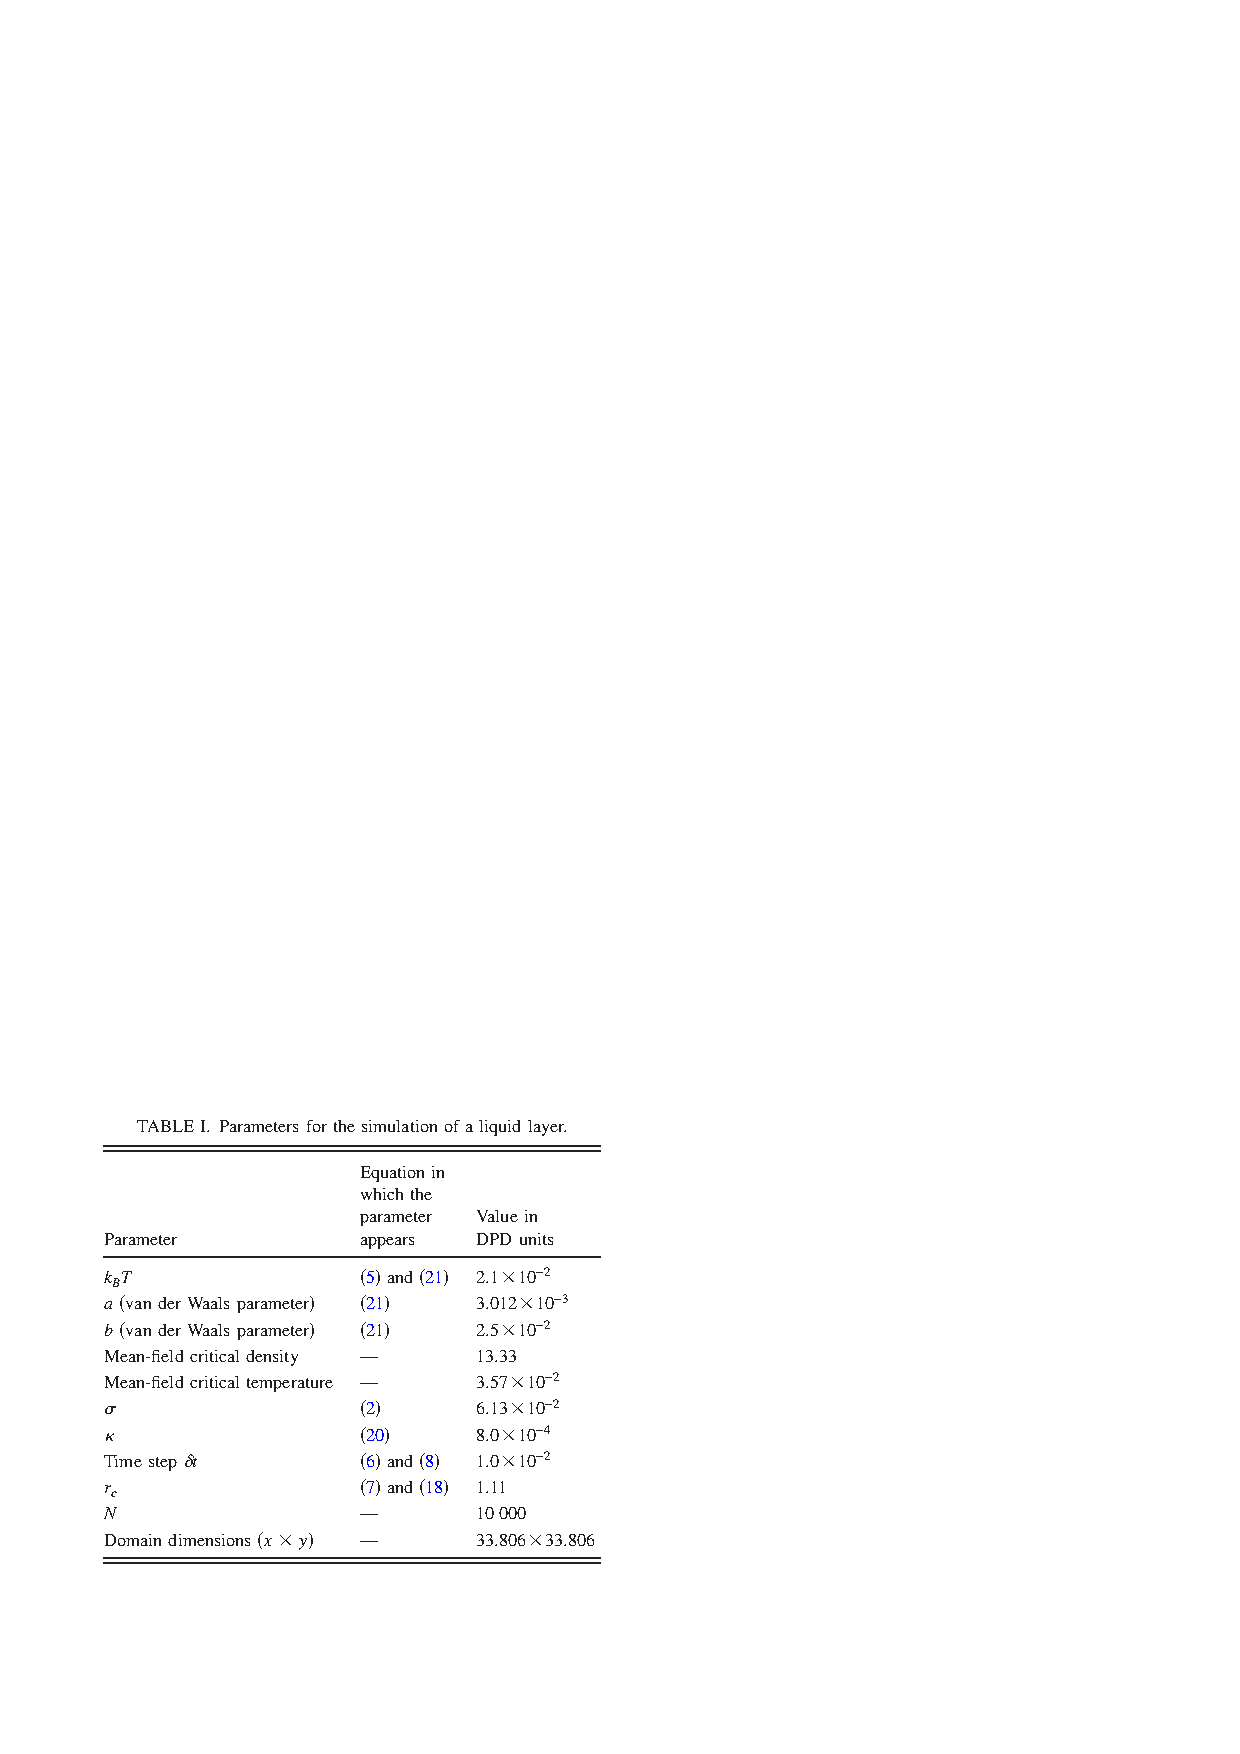
\includegraphics[width=1\textwidth]{./figures/parameter.pdf}
\end{center}
\end{column}
\end{columns}
}

\frame{\frametitle{表面张力的计算}
\begin{columns}
\begin{column}[c]{0.5\textwidth}
\begin{center}
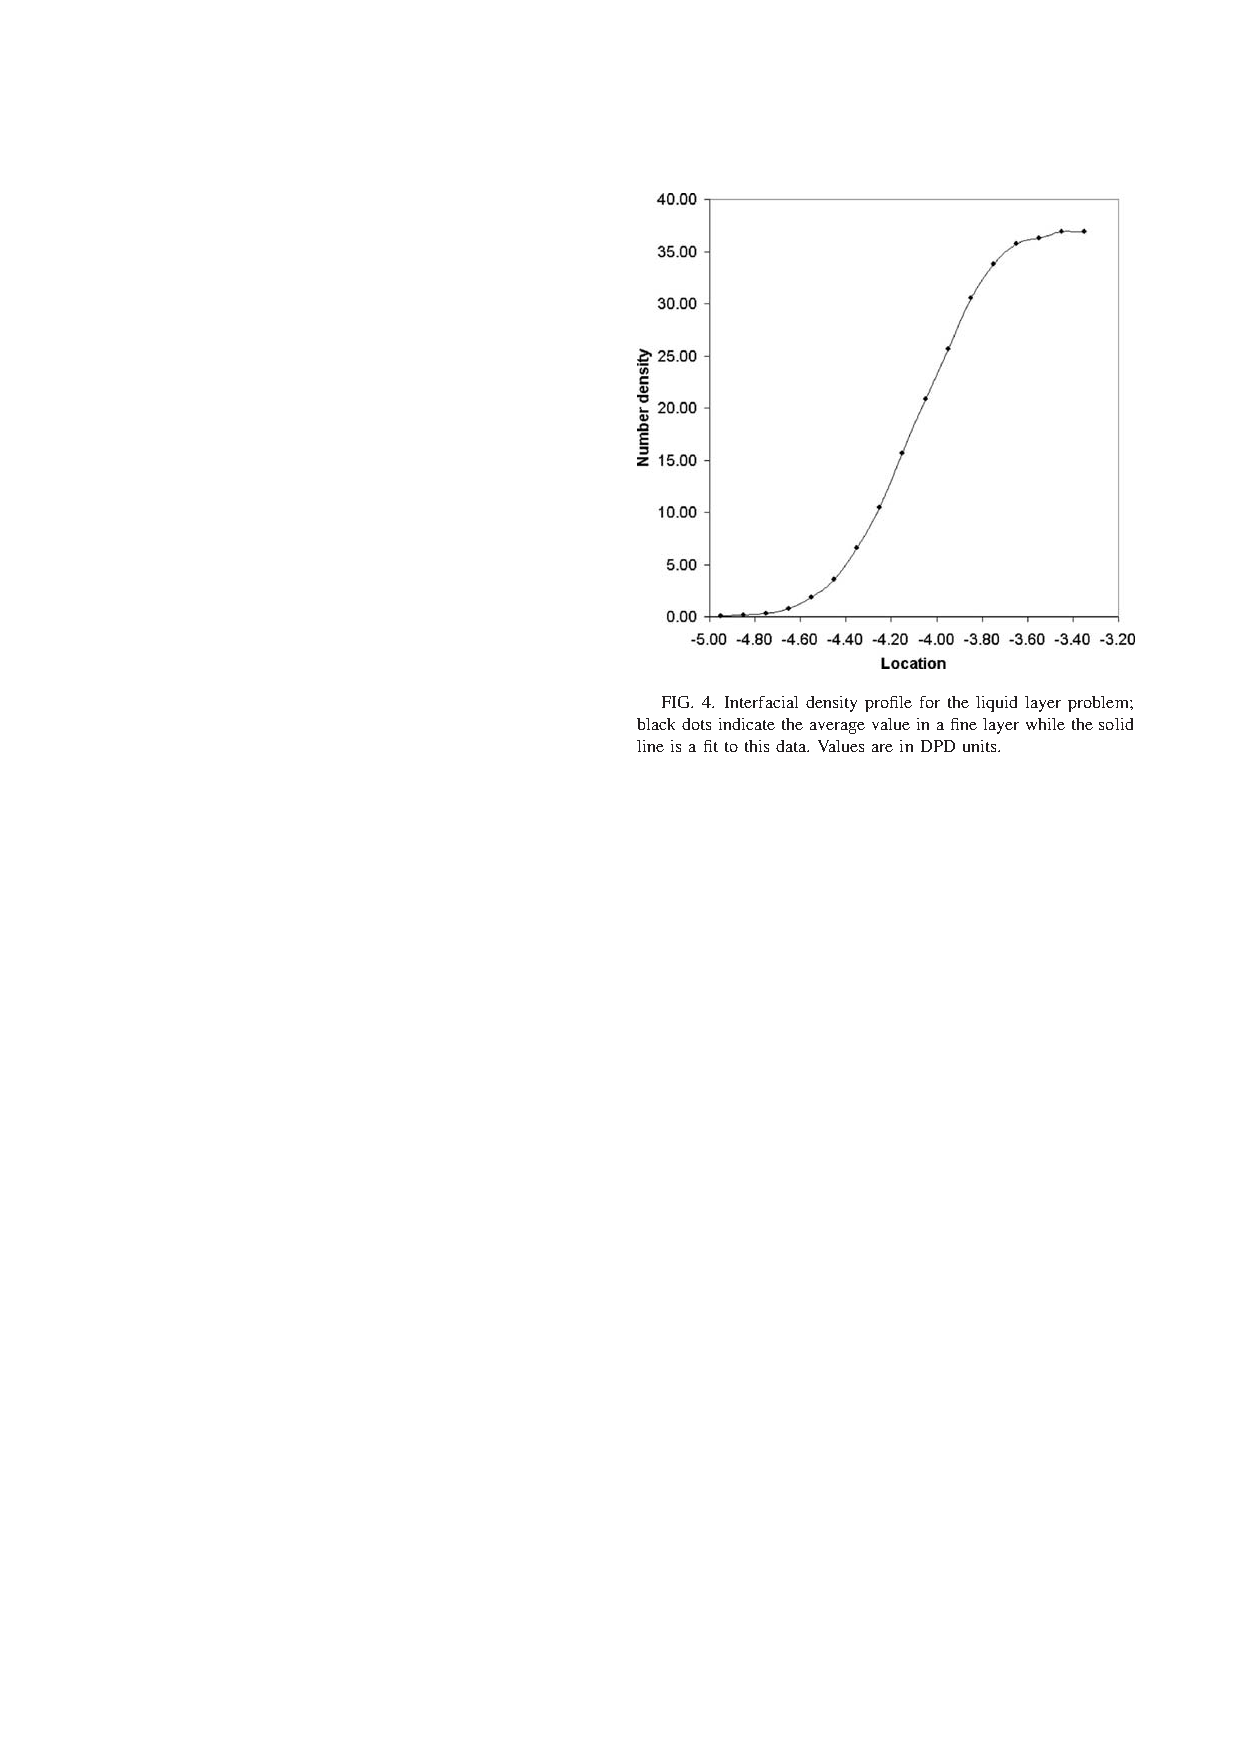
\includegraphics[width=1\textwidth]{./figures/density.pdf}
\end{center}
\end{column}
\begin{column}[c]{0.5\textwidth}
表面张力计算公式:
\[
\sigma_s=\kappa \int_{-\infty}^{+\infty}\Big(\frac{\partial \rho}{\partial n}\Big)dn
\]
\end{column}
\end{columns}
}

\subsection{Laplace law simulations}

\frame{\frametitle{结构与计算方法}
\begin{columns}
\begin{column}[c]{0.5\textwidth}
\begin{center}
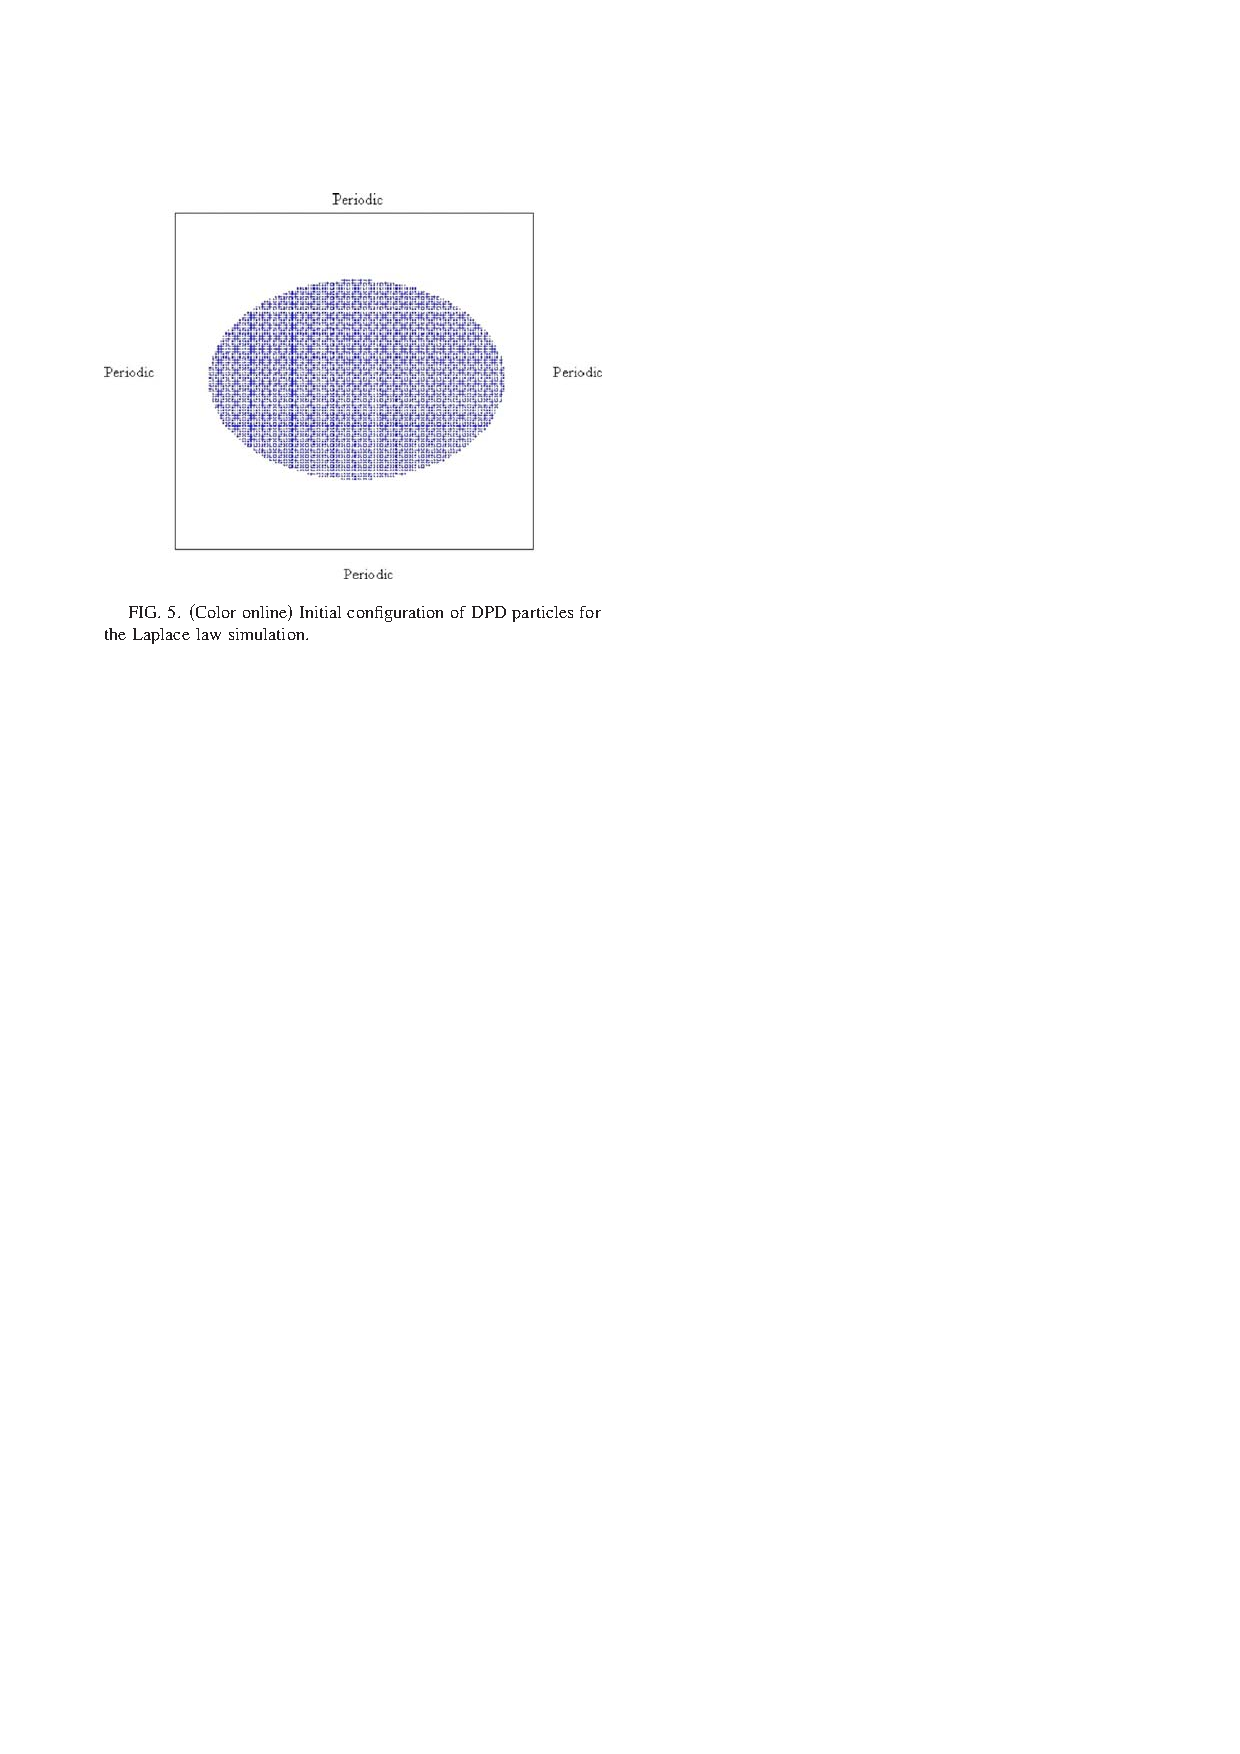
\includegraphics[width=1\textwidth]{./figures/configuration2.pdf}
\end{center}
\end{column}
\begin{column}[c]{0.5\textwidth}
二维的Laplace law 如下:
\[
p_{in}-p_{out}=\frac{\sigma_s}{R}
\]
压强和曲率半径的计算:
\[
p=\rho k_BT+\frac{1}{2dV}\sum_i\sum_jr_{ij}F_{ij}^C
\]

\[
R=\sqrt{N/(\pi\rho_{eq})}
\]
\end{column}
\end{columns}
}

\frame{\frametitle{Laplace law的证明}
\begin{center}
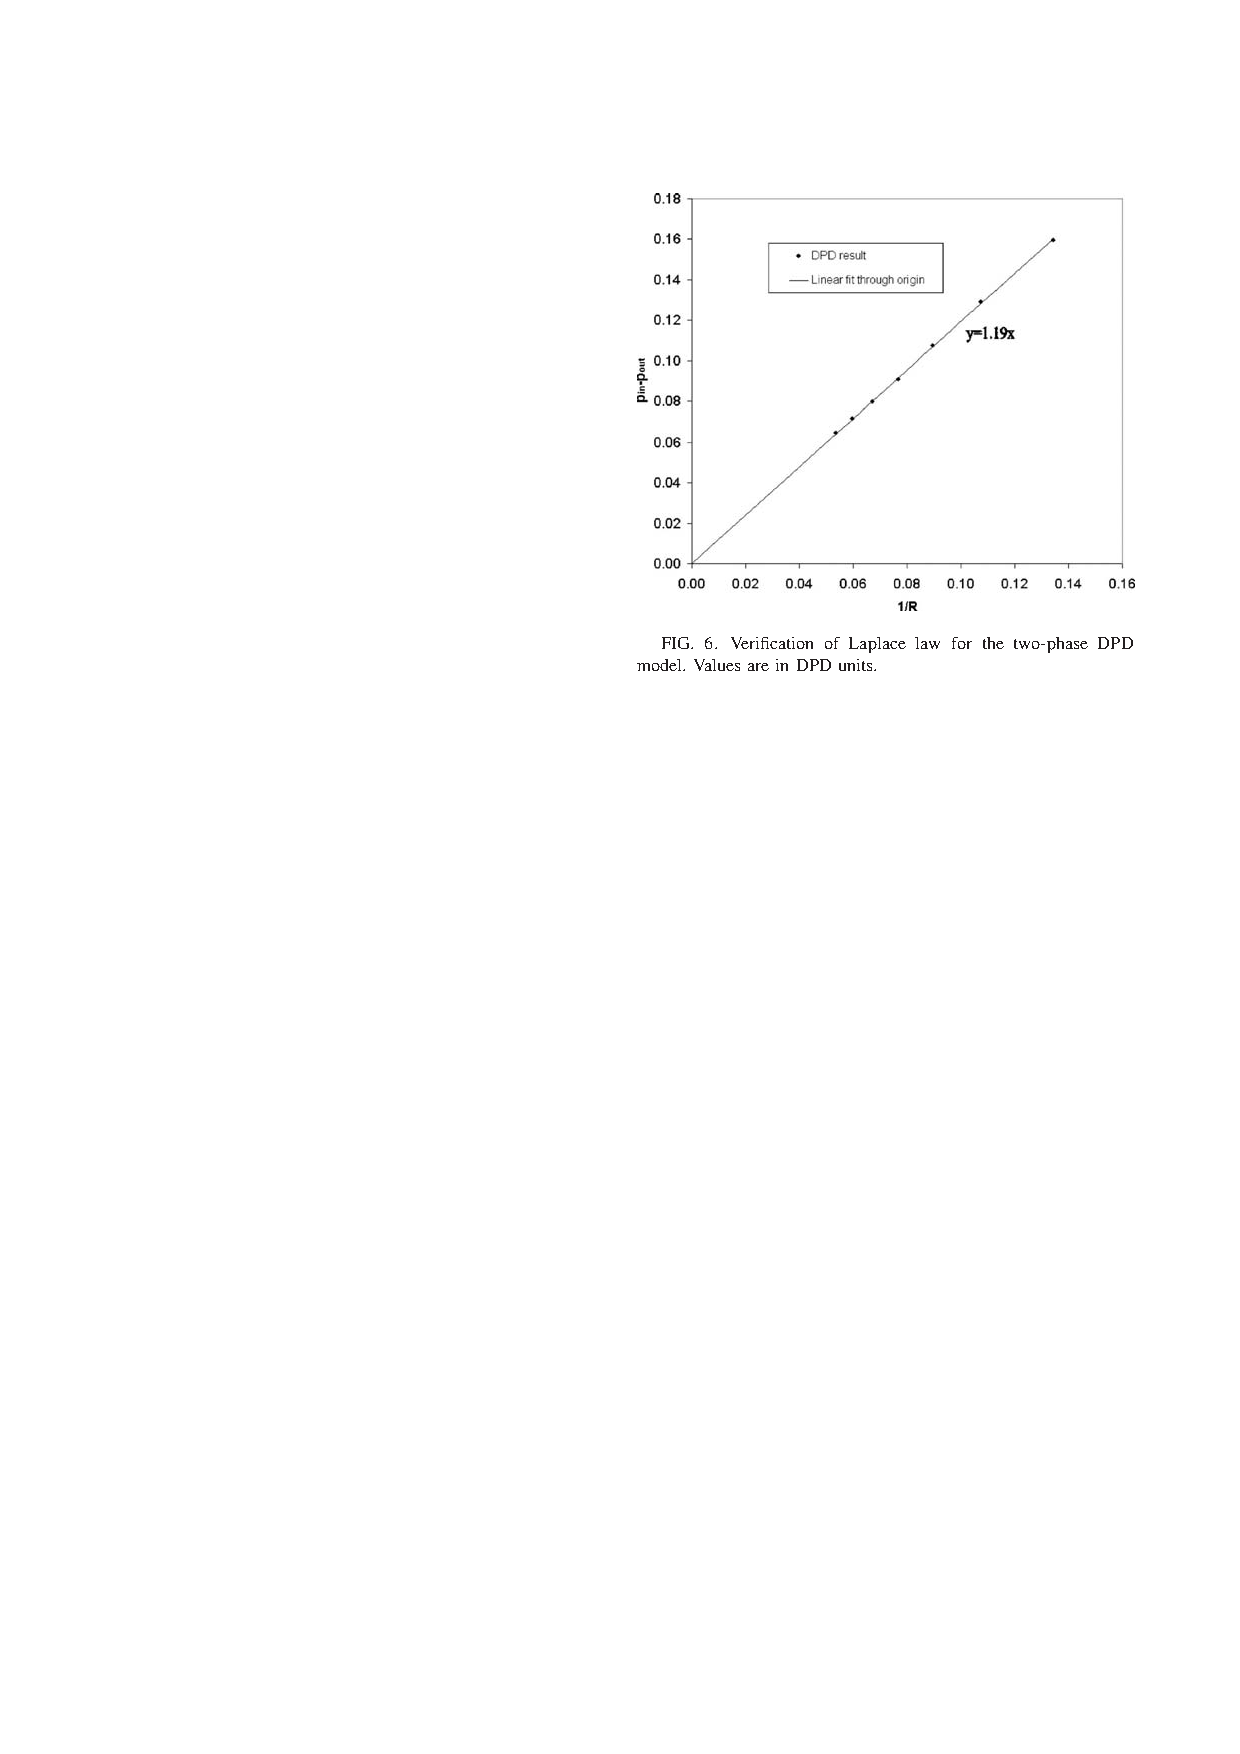
\includegraphics[width=0.6\textwidth]{./figures/verificationLaplace.pdf}
\end{center}
}

\subsection{Ocillation of a liquid cylinder}

\frame{\frametitle{Small-amplitude oscillations}
\begin{columns}
\begin{column}[c]{0.5\textwidth}
\begin{center}
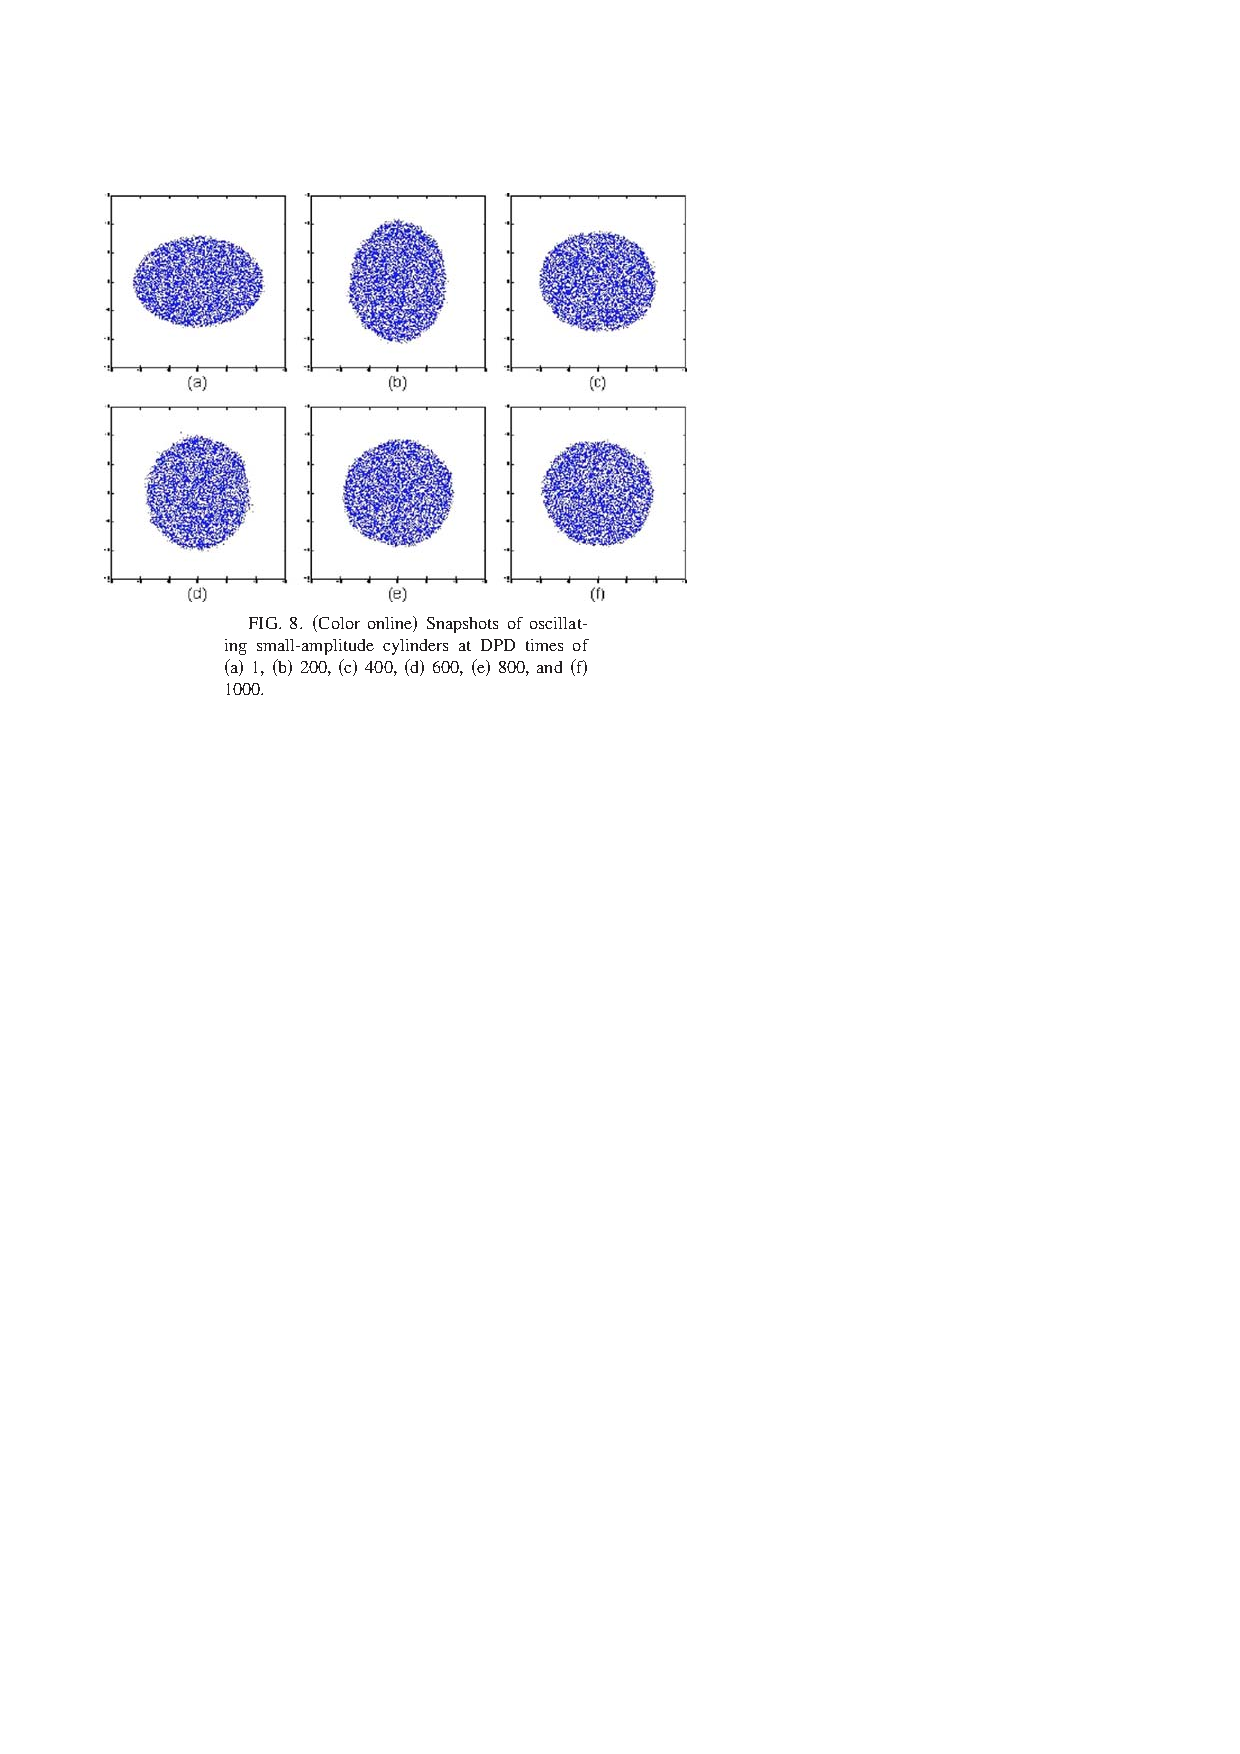
\includegraphics[width=1\textwidth]{./figures/oscillate.pdf}
\end{center}
\end{column}
\begin{column}[c]{0.5\textwidth}
\begin{center}
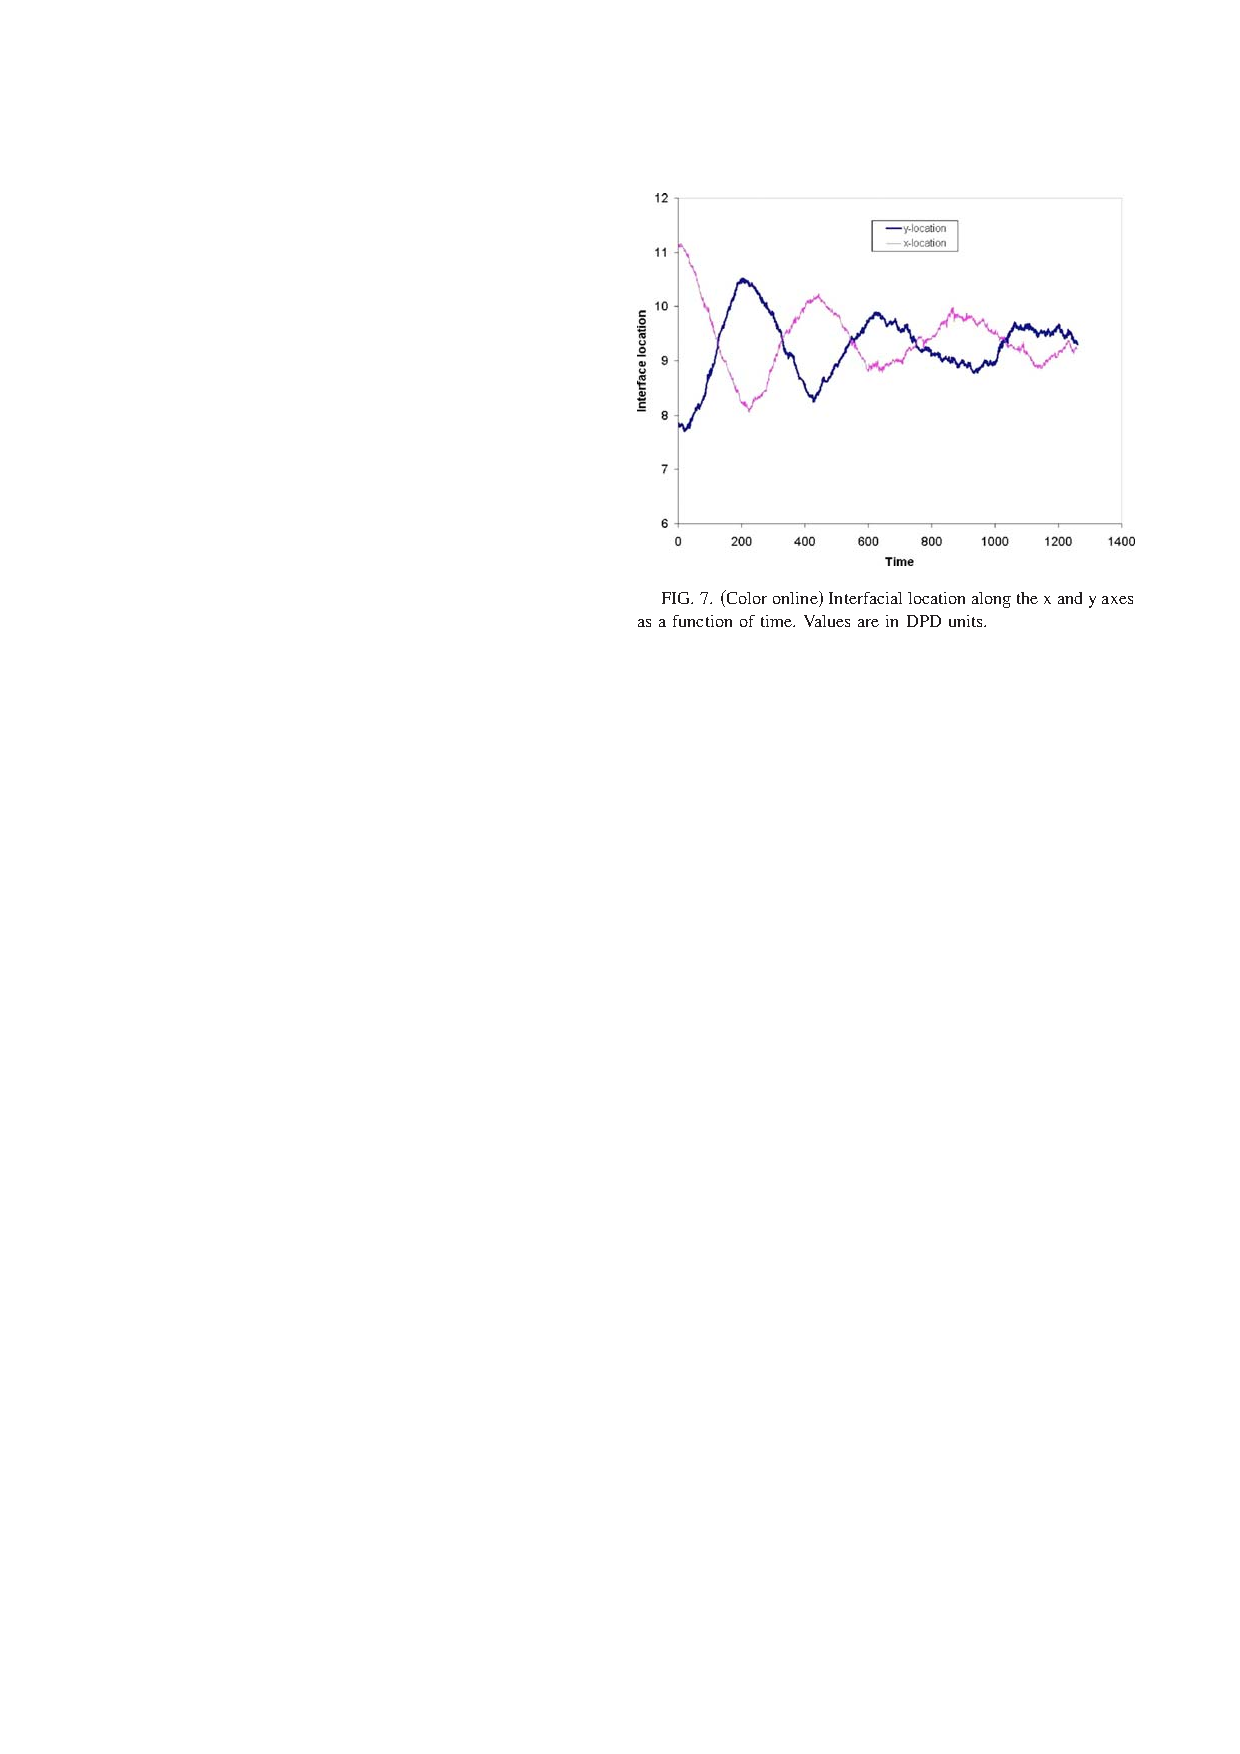
\includegraphics[width=1\textwidth]{./figures/InterfaceLocation.pdf}
\end{center}
\end{column}
\end{columns}
}

\frame{\frametitle{Large-amplitude oscillations}

\begin{center}
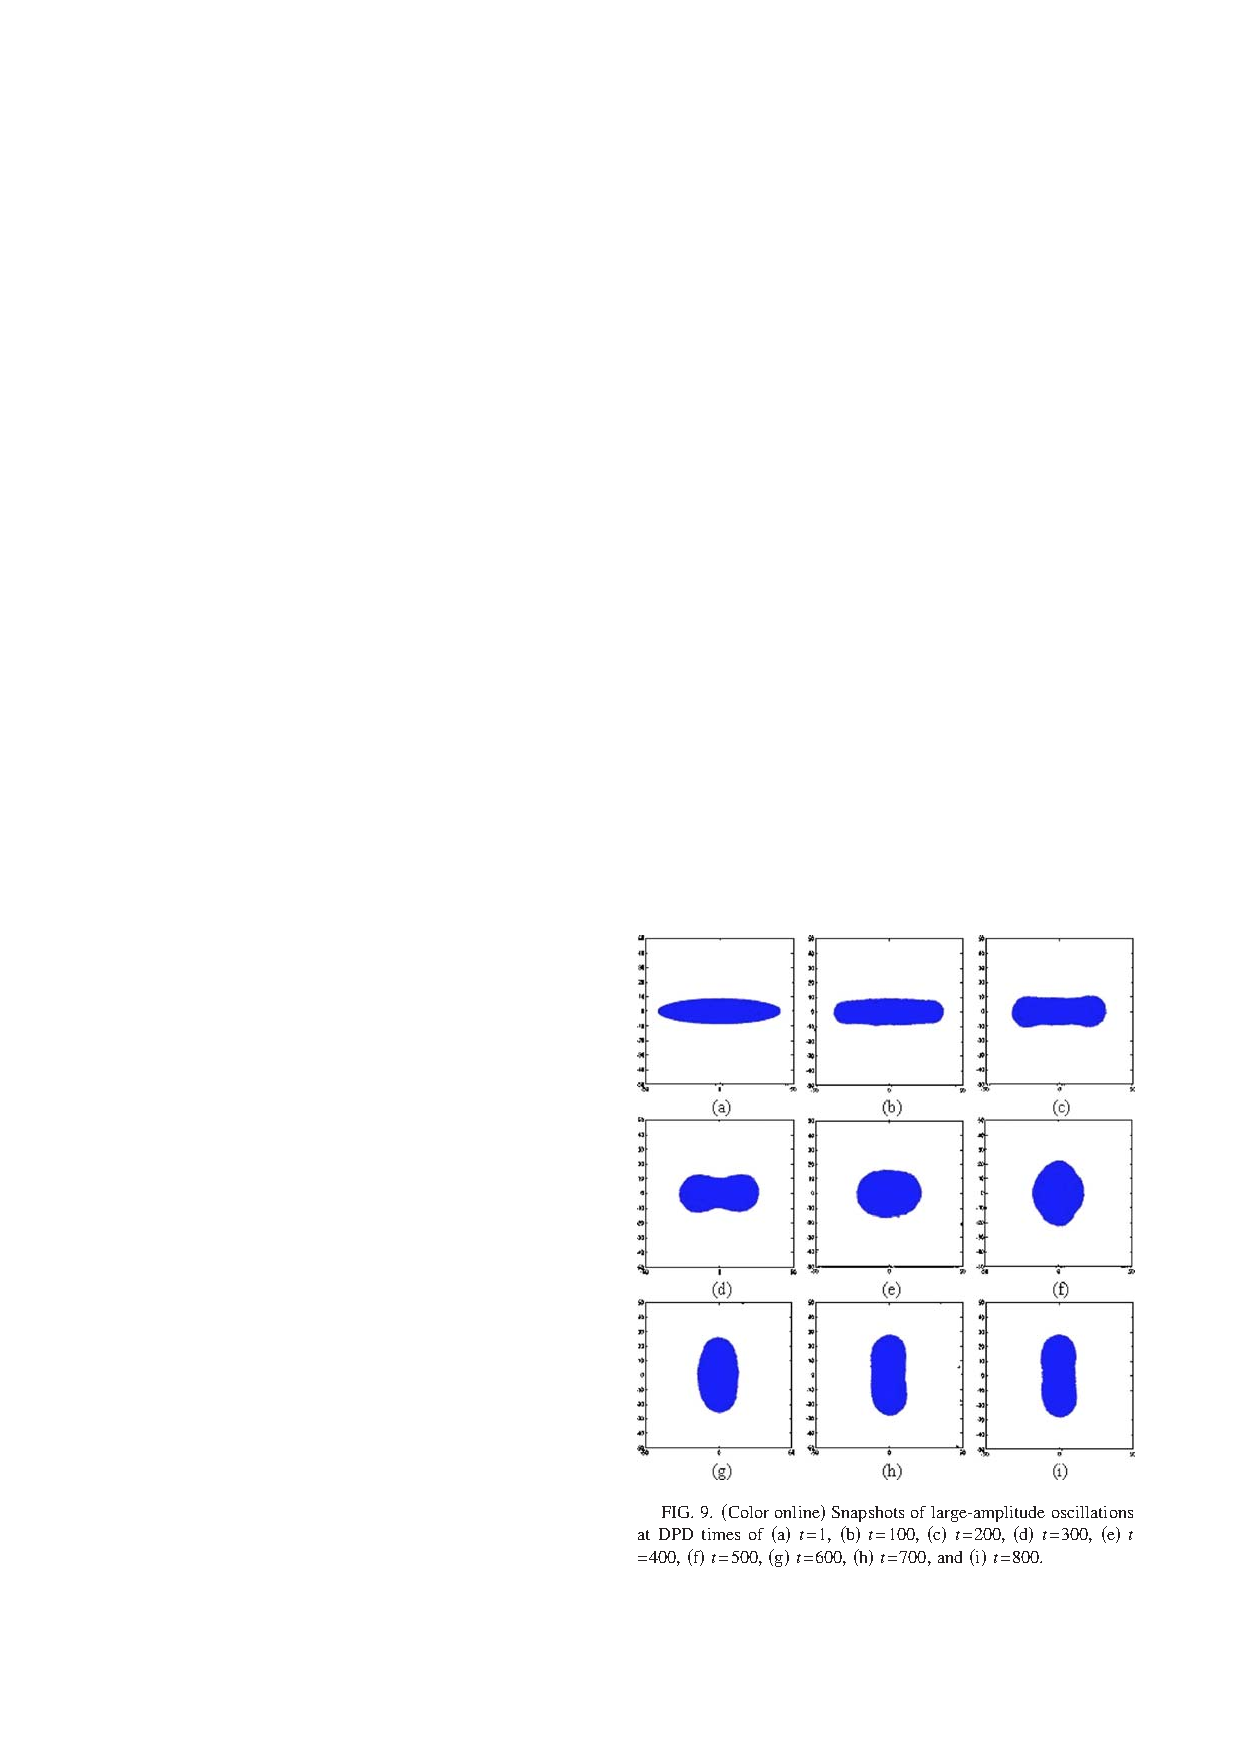
\includegraphics[width=0.5\textwidth]{./figures/LargeAmplitude.pdf}
\end{center}
}



\newcount\opaqueness
\plainframe{
    \begin{centering}
      \Huge Thank You!!!\par
    \end{centering}
} 


\end{document}
